\documentclass{article}
\usepackage[a4paper, total={6in, 8in}, margin=20mm]{geometry}
\usepackage{graphicx}
\usepackage{hyperref}
\parindent=0pt
\parskip=12pt

\begin{document}
	The OPTIMADE API enables a user to obtain material information from multiple providers with the same filter query. This is particularly useful for machine learning workflows. Being able to query multiple providers using a single API allows a user to combine data from multiple sources, each of which may have different ``strengths''. Below, we describe the use of the OPTIMADE API in an exemplar machine learning workflow.
	
	We used the OPTIMADE API to retrieve high-entropy alloy materials using the filter query 
	\begin{quote}
		`elements HAS ANY ``W",``Al",``Cd",``Zn" AND NOT elements HAS ANY ``B", ``Cl", ``F", ``H", ``N", ``O", ``S", ``Se" AND nelements$>$=5'		
	\end{quote}
	from three different providers (anonymized as P1, P2, P3). The number of materials returned by each provider and a Venn diagram of unique elements that appear in the materials from each provider are shown in the bottom inset in \autoref{fig: exampleFig}.

	Standard structural entries of the OPTIMADE specification, \verb|species_at_sites| and \verb|lattice_vectors|, are used to calculate the densities of the materials. Vectors codifying the composition of each material are also constructed. These vectors are used as inputs to machine learning models which are trained to predict the densities (outputs).
	
	We choose a Random Forest Regressor (from the \verb|scikit-learn| package in Python) to construct the machine learning models for our example. If data from a only one provider is used for training a model but tested on data from all the providers, the model does not perform very well. We can see this from the scatter plot of predicted and actual density values in \autoref{fig: exampleFig} for small sample of data-points. For models trained only on data from a single provider (M-P1, M-P2 and M-P3), the prediction is quite accurate when tested on data from the same provider (indicted by `cross' markers). However, most of the predictive power is lost when tested on data from another provider (`dot' markers). Meanwhile, the model which is trained on data from all providers (C) retains its predictive power when tested on data from all the providers. A comparison of the R$^2$ values shown in the top-left inset confirms this.
	
	The complete dataset is split into training and testing sets (4:1 ratio) while ensuring that ratio of entries from each provider is the same in both training and testing sets. This is used to train the model M-C. To train M-P1, M-P2, M-P3, data-points from the corresponding provider which appear in the training set are used. Scoring of each of the models is carried out using the same test set. 
%	A model trained on data from all the providers (say C) performs quite well when tested on materials from any of the three providers. On the other hand, i
%	
%	When this model is trained on data from all the providers, it performs quite well (R$^2 = 0.98$, see top inset in \autoref{fig: exampleFig}) 
%	
%	
%	than when it is trained on data from only one provider when tested on data from the same pool.  Meanwhile, the model trained on data from call providers (C) retains its predictive power for data from all the providers.
	
	

	\begin{figure}[h]
		\centering
		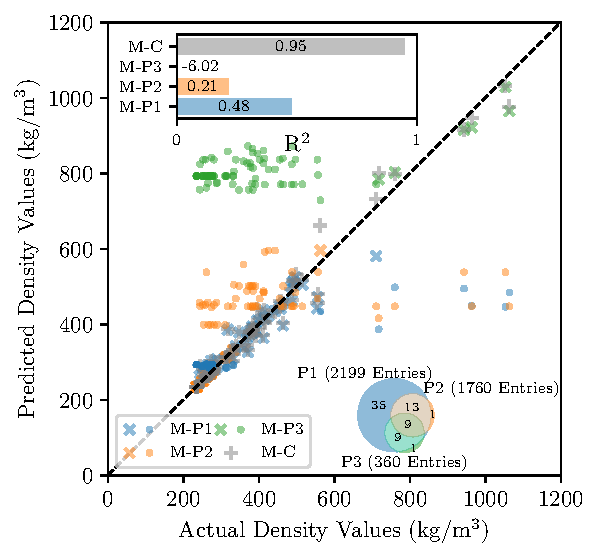
\includegraphics[]{scatterPlot.pdf}
		\caption{} 
		\label{fig: exampleFig}
	\end{figure}
\end{document}